%!TeX root=../tese.tex
%(dica para o editor de texto: este arquivo é parte de um documento maior)
% para saber mais: https://tex.stackexchange.com/q/78101/183146

\chapter{Redes neurais no contexto de aprendizado de máquina}
\label{cap:redes}

Neste capítulo são apresentados alguns conceitos básicos de ciência de dados e de aprendizado de máquina, alguns dentre os vários tipos e exemplos de algoritmos de aprendizagem, direcionando-os para aquele que é o foco do trabalho, ou seja, as redes neurais artificiais.

Neste texto os termos ``algoritmo'' e ``técnica'' serão usados livremente como sinônimos, pois uma técnica de aprendizado de máquina, no contexto atual, é um algoritmo executado no computador que tem por objetivo ajustar parâmetros de modelos estatísticos.

Analogamente à definição dada na Introdução (\ref{cap:introducao}), citamos outras duas. Prince Barpaga \citep{prince} define aprendizado de máquina como sendo um ramo da inteligência artificial, em que computadores são treinados a partir de dados conhecidos para realizar alguma tarefa específica, ao invés de ser explicitamente programado para exibir uma resposta fixa.

Similarmente, Robbie Allen \citep{allen} descreve que um conjunto de dados é usado para treinar um modelo estatístico de forma que, ao ser deparado com dados similares aos dados usados para o treino, saberá como tratá-los. Geralmente, dados são usados como entradas para esses modelos que irão fornecer como saída predições de interesse.

Concluindo, pode-se utilizar o grau de supervisão humana durante o aprendizado para classificá-los em diferentes tipos, como é descrito por Géron \citep{hands}. Durante o aprendizado podem ser fornecidos um conjunto de consultas e de respostas já conhecidas. Tais respostas foram dadas por humanos, ao menos neste momento, e daí o termo ``supervisão humana''.

\section{Tipos de aprendizagem}

Um algoritmo de \defi{aprendizado supervisionado} é usado quando conhecemos características dos dados que estamos utilizando. De modo geral já temos de antemão as respostas às consultas para os dados utilizados no treinamento. Por exemplo, se estamos classificando fotos de animais, possuímos um conjunto de fotos para as quais já sabemos quais são de gatos, cachorros, etc.

O ato de rotular previamente os dados que usamos no treinamento é o que designamos de supervisão humana. Uma vez \emph{treinado}, o algoritmo recebe uma foto, ou seja, uma nova consulta e então fornece a resposta, neste caso se essa é a foto de um gato, ou cachorro, ou qualquer outra resposta dentre aquelas que foram dadas como exemplos durante o treinamento.

Dentro do aprendizado supervisionado temos duas técnicas principais. A primeira é a \defi{classificação}, usada para rotular ou dividir os dados em classes pré-determinadas, a partir de exemplos, que é exatamente o caso dos exemplos descritos nos parágrafos anteriores, e ilustrada na figura \ref{fig:classify}.

\begin{figure}[htb]
\centering
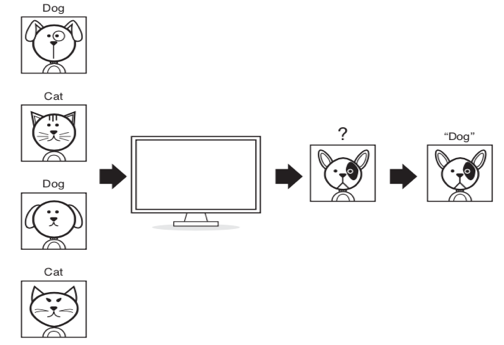
\includegraphics[width=8cm]{figuras/classificacao}
\caption{Tarefa de classificação.\footnote{Extraído de \citep{allen}}}
\label{fig:classify}
\end{figure}

A segunda técnica é a \defi{regressão}, usada para prever valores, ou seja, fornecer respostas a consultas ainda inéditas, sejam dados do futuro ou valores de funções em pontos do domínio para os quais ainda não existem valores. Podemos entender a diferença, com a ajuda de Allen \citep{allen} se percebermos que na classificação as respostas são valores discretos, isto é, um `cachorro' ou um `gato'. 

Enquanto isso, na regressão as respostas são valores contínuos, um intervalo real de possibilidades. Como exemplo, Allen \citep{allen} ilustra na figura \ref{fig:regressao}, dado uma imagem radiológica, um modelo poderia prever em quantos anos uma pessoa poderia desenvolver alguma doença.

\begin{figure}[htb]
\centering
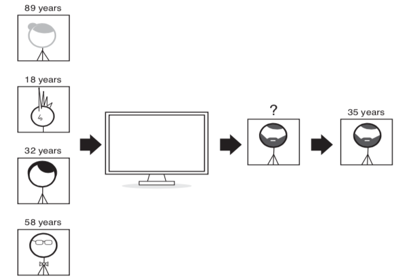
\includegraphics[width=8cm]{figuras/regressao}
\caption{Tarefa de regressão.\footnote{Extraído de \citep{allen}}}
\label{fig:regressao}
\end{figure}

No \defi{aprendizado não-supervisionado} não sabemos os rótulos dos dados que estamos lidando, isto é, não sabemos previamente respostas aos dados conhecidos, assim o algoritmo poderá agrupar os dados de forma automática, por exemplo, se estivermos lidando com problemas de classificação. Aqui, as consultas podem ser coisas como ``quantos são os perfis dos clientes'' ou ``quantas espécies de flores existem nestas fotos'', e assim por diante.

Alguns métodos não-supervisionados de aprendizado foram enumeradas por Géron \citep{hands}. O \defi{agrupamento} de dados similares sob uma inspiração geométrica. Nesse caso os dados são agrupados conforme suas posições num determinado espaço e utiliza-se algoritmos como $k$-vizinhos, $k$-means, $k$-medians, etc. Exemplos de aplicações são agrupamento de produtos em supermercados, interesses comuns de clientes em sites de conteúdo digital, etc.

Para ilustar, Allen \citep{allen} sugere que imaginemos um conjunto de artigos de texto que gostaríamos de organizar. Alguns poderiam ser sobre esportes, outros sobre história, outros sobre arte, etc. O objetivo seria identificar e classificar automaticamente os textos dentre alguns assuntos possíveis. Imaginando cada assunto provável como uma figura geométrica diferente, a tarefa seria realizada idealmente como na figura \ref{fig:clustering}.\footnote{Vale ressaltar que não sabemos \emph{a priori} os rótulos aqui representados a favor do entendimento.}

\begin{figure}[htb]
\centering
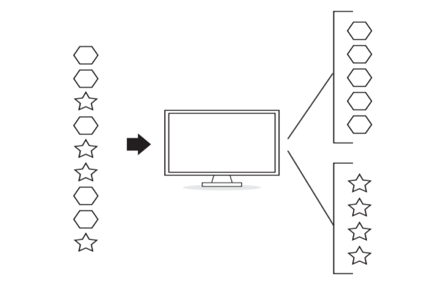
\includegraphics[width=8cm]{figuras/clustering}
\caption{Tarefa de clusterização.\footnote{Extraído de \citep{allen}}}
\label{fig:clustering}
\end{figure}

Existe também o \defi{aprendizado semi-supervisionado} em que combinam-se vantagens de ambos os tipos anteriores. Um modelo utiliza dados sem rótulos para descobrir uma estrutura geral dos dados, enquanto usa alguns poucos rótulos conhecidos para ajudar na organização inicial dessa estrutura, o que auxilia na partida do agrupamento, que é um problema das técnicas não-supervisionadas.

Essa técnica é também conhecida por \emph{aprendizagem fraca}, e conforme aponta Allen \citep{allen} possui a vantagem de precisar de menor quantidade de dados rotulados para que se alcançe um bom resultado em termos de qualidade do modelo, já que aprende parte do padrão dos dados a partir dos dados sem rótulos.

Uma técnica já bem diferente das anteriores, é o \defi{aprendizado por reforço}. Allen \citep{allen} nos explica o conceito principal dessa abordagem, que consiste na existência de um ``agente'' que interage executando ações num ``ambiente'', que por sua vez dá um retorno (\eng{feedback}) a esse agente, usualmente na forma de uma ``recompensa''.

Tal recompensa pode ser entendida especificamente como um contador. O objetivo do agente é maximizar esse contador. Nenhuma informação é dita ao agente sobre como ele aumenta esse contador, ou porquê ele conseguiu aumentar, ele irá definir suas ações de acordo com as respostas dadas pelo ambiente. 

Assim, tudo que ele sabe é se houve a recompensa ou não, e irá preferir as ações que fizeram o contador aumentar e preterir aquelas que fizeram ele diminuir, sem nunca existir rótulos ou respostas esperadas.

Outra técnica é a \defi{detecção de anomalias}, cujo objetivo é ter uma descrição de como os dados considerados ``normais'' se parecem, e usa-se esse agrupamento para detectar se novos dados estariam ``fora'' desse padrão. Um exemplo é a detecção de fraudes.

Também pode-se citar a técnica de \defi{estimação de densidades}, que tem como objetivo a estimação da função densidade de probabilidade de um conjunto de dados gerados por algum processo aleatório.

\subsection{O problema do sobreajuste dos modelos}

O sobreajuste (\eng{overfitting}) é o primeiro desafio que deve ser enfrentado quando realizados uma tarefa de aprendizado de máquina. Um modelo de aprendizado de máquina só é considerado válido ou útil, se ele chega a um ponto de existir nenhum ou muito pouco sobreajuste.

O sobreajuste ocorre quando um modelo foi treinado exageradamente para o conjunto de dados conhecidos, ou seja, o conjunto utilizado para o treino. De forma que, ao se deparar com dados novos, desconhecidos, perde a capacidade de saber o que fazer, ou seja, erra muito nas previsões. 

Isto pode ocorrer tanto nas tarefas de classificação, quanto nas tarefas de regressão. Utilizando o exemplo dado por Allen \citep{allen}, imaginemos um modelo de classificação de fotos de animais. Um modelo $100\%$ sobreajustado irá \emph{decorar} as cores de cada um dos pixels dessa imagem, de forma que todos eles serão necessários para ele identificar se tal foto é um gato, ou um cachorro, etc.

Mudando apenas a cor ou a posição de um dos pixels de uma das imagens, e supondo que essa imagem modificada não fazia parte do conjunto de imagens do treinamento, o modelo não será capaz de fornecer uma resposta válida ou confiável. A figura \ref{fig:over_class} ilustra esse exemplo.

\begin{figure}[htb]
\centering
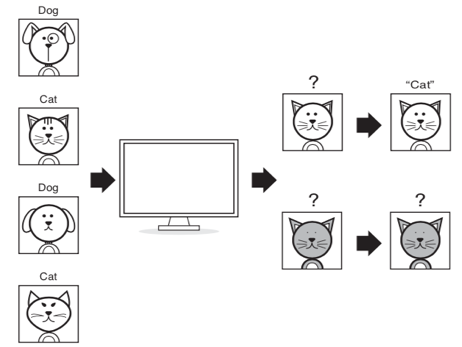
\includegraphics[width=8cm]{figuras/over_class}
\caption{Sobreajuste num modelo de classificação.\footnote{Extraído de \citep{allen}}}
\label{fig:over_class}
\end{figure}

Isto é o sobreajuste, o modelo fica perfeito para os dados de treino, mas fica totalmente cego para os dados do mundo real, desconhecidos. Ele também está presente nos modelos de regressão. Consideremos o exemplo dado por Allen \citep{allen}.

Seja um gráfico que relaciona a metragem ao quadrado de terrenos, no eixo $X$ com o valor pago por eventuais compradores, no eixo $Y$. É um típico problema de regressão, já que queremos saber, para metragens de terrenos ainda desconhecidos, qual um valor esperado para sua compra ou venda. 

O modelo mais simples seria o de uma regressão linear, explicado em detalhes na próxima seção, em que basicamente, traçamos uma reta do tipo $y = bx + a$, cujo valor $y$ irá servir de valor esperado para nosso modelo, para qualquer $x$ ainda desconhecido. Uma ilustração desse modelo hipotético está na figura \ref{fig:over_reg_1}.

\begin{figure}[htb]
\centering
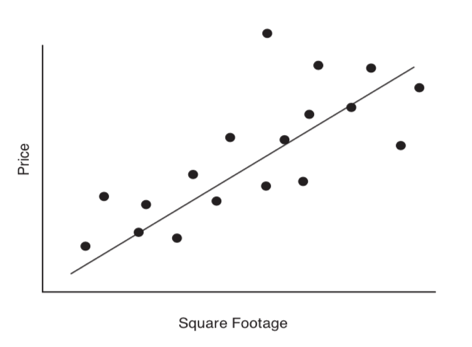
\includegraphics[width=8cm]{figuras/over_reg_1}
\caption{Modelo de regressão, ajuste linear.\footnote{Extraído de \citep{allen}}}
\label{fig:over_reg_1}
\end{figure}

Podemos não ficar satisfeitos com esse ajuste linear, já que praticamente nenhum ponto está contido perfeitamente na reta ajustada. E assim, supomos um novo modelo, dessa vez de um polinômio quadrático, isto é, um modelo do tipo $y = cx^2 + bx + a$. 

A diferença é que antes tínhamos $2$ parâmetros para ajustar, $a$ e $b$, e agora temos um terceiro parâmetro, $c$.\footnote{É importante mencionar que, em outros contextos, o número de parâmetros livres de um modelo é conhecido como o número de \emph{graus de liberdade} desse modelo.} Um ajuste possível, é ilustrado na figura \ref{fig:over_reg_2}.

\begin{figure}[htb]
\centering
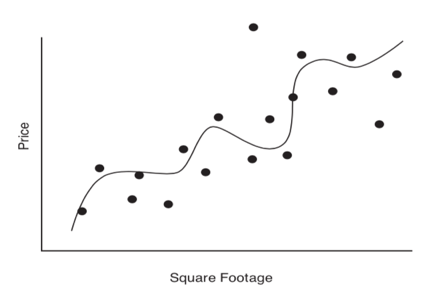
\includegraphics[width=8cm]{figuras/over_reg_2}
\caption{Modelo de regressão, polinômio quadrático.\footnote{Extraído de \citep{allen}}}
\label{fig:over_reg_2}
\end{figure}

Aparentemente, esse modelo é melhor do que o anterior, pois a função está melhor ajustada aos dados conhecidos. Poderíamos pensar que quanto mais parâmetros, isto é, quanto maior o grau do polinômio a ser ajustado, mais adequado o modelo estará aos dados. 

Isso pode chegar até o extremo em que, possuindo $n{+}1$ dados, tentamos ajustar um polinômio de grau $n$. Tal ajuste está ilustrado na figura \ref{fig:over_reg_3}.

\begin{figure}[htb]
\centering
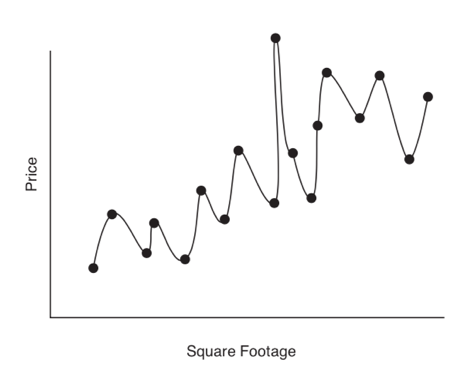
\includegraphics[width=8cm]{figuras/over_reg_3}
\caption{Modelo de regressão, polinômio de grau $n$.\footnote{Extraído de \citep{allen}}}
\label{fig:over_reg_3}
\end{figure}

Com isso, teremos o caso extremo de um modelo de regressão $100\%$ sobreajustado. Ele está perfeitamente ajustado aos dados conhecidos, mas retornará resultados espúrios para qualquer outro $x$ que não pertença a esse conjunto, perdendo totalmente a capacidade de \emph{generalização}, conforme explicado por Allen \citep{allen}.

O objetivo dessa discussão é apontar que devemos ser parcimoniosos na escolha do nosso modelo, tentando buscar o menor número possível de parâmetros a serem corretamente ajustados, de modo a dar ao mesmo tempo uma boa perfomance no conjunto de treinamento (mas não perfeita), e também uma capacidade igualmente boa de generalização para os dados desconhecidos.

\section{Alguns algoritmos de aprendizagem}

Conhecendo os tipos mais comuns de aprendizagem, o próximo passo nesse caminho da ciência de dados é conhecer os diferentes algoritmos de aprendizagem, alguns sendo mais usados em tarefas supervisionadas, outros em tarefas não-supervisionadas e alguns podendo ser utilizados em ambos os tipos de tarefas.

É importante também conhecer para quais tarefas do mundo real eles foram concebidos, pois essa etapa é muito importante, dentro do contexto humano da ciência de dados, para se adquirir intuição e auxiliar na escolha do algoritmo ou dos algoritmos mais úteis que possam modelar algum novo problema.

\subsection{Regressão Linear}

Um dos pioneiros e mais simples problemas de aprendizagem de máquina supervisionada. É, aliás, um método nascido e desenvolvido na \emph{estatística}, possuindo soluções fechadas, como por exemplo o método dos mínimos quadrados. 

Porém, o uso de técnicas computacionais é muito bem-vinda, se estamos lidando com volumes de dados muito grandes, e que exigem manipulações aritméticas de matrizes, como multiplicação, inversão, diagonalização, etc.

Formalmente, supomos um modelo de regressão linear múltipla, associando um conjunto de variáveis independentes $X_1, X_2, \ldots, X_p$, que representam os dados, a uma variável dependente $Y$, que representa a resposta esperada, escrevemos o seguinte modelo.

\begin{equation}\label{algo:1}
Y = \E(Y|X_1 = x_1, \ldots, X_p = x_p) + \epsilon = \beta_0 + \beta_1 X_1 + \ldots + \beta_p X_p + \epsilon
\end{equation}
onde $\epsilon$ é o erro aleatório, para o qual é assumido uma distribuição normal de média $0$.

Temos portanto $p{+}1$ parâmetros a serem ajustados em nosso modelo. Uma solução conhecida para o caso univariado, retirada de Magalhães e Lima \citep{antonio} (páginas $332{-}336$), e que pode ser generalizada, é dada pelo método dos mínimos quadrados. 

Se possuímos $n$ observações disponíveis, tanto das variáveis independentes $X_i$ quanto das variáveis dependentes $Y_i$, e denotando da seguinte maneira:

\[
Y = \left[ \begin{array}{c} Y_1 \\ Y_2 \\ \vdots \\ Y_n \end{array} \right], \;
X = \left[ \begin{array}{cccc} 1 & x_{11} & \ldots & x_{1p} \\ 1 & x_{21} & \ldots & x_{2p} \\ \vdots & \vdots & \ddots & \vdots \\ 1 & x_{n1} & \ldots & x_{np} \end{array} \right], \;
\beta = \left[ \begin{array}{c} \beta_0 \\ \beta_1 \\ \vdots \\ \beta_p \end{array} \right], \;
\epsilon = \left[ \begin{array}{c} \epsilon_1 \\ \epsilon_2 \\ \vdots \\ \epsilon_n \end{array} \right]
\]

Usando essa notação, podemos reescrever a equação (\ref{algo:1}), para $n$ observações:

\begin{equation}\label{algo:2}
Y = X \beta + \epsilon
\end{equation}

Esse problema possui uma solução algébrica dada pelo método dos mínimos quadrados, que nos fornece uma estimativa do vetor $\beta$, que é:

\begin{equation}\label{algo:3}
\hat{\beta} = (X'X)^{-1}X'Y
\end{equation}

Que envolvem as operações de matrizes mencionadas acima. E que assume uma definição baseada na minimização da função de erro quadrático, feita de forma algébrica. 

As técnicas de aprendizado de máquina entram em jogo se queremos utilizar uma outra função de erro, ou se queremos uma outra abordagem para a minimização da função de erro escolhida, como por exemplo o método do gradiente descendente, explicado em detalhes no Apêndice \ref{ap:gradiente}.

A utilização do gradiente descendente ou de outro método de otimização qualquer é motivado pela maior eficiência computacional desses métodos em comparação com a inversão de matrizes de ordem $p{\times}p$ necessária no cálculo direto de \ref{algo:3}. A justificativa é facilmente verificada em problemas do mundo real, onde, na maioria dos casos, $p{>}1.000$.

Outras técnicas também podem ser utilizadas quando estamos no contexto de aprendizado de máquina. Daniil Korbut \citep{korbut} citam as técnicas de regularização, que são úteis para se evitar o sobreajuste nos modelos de regressão. 

A ideia da regularização é adicionar parâmetros sem importância prática às somas dos quadrados na função de erro quadrático, com o objetivo de minimizar os valores dos parâmetros de interesse. Explicações mais detalhadas podem ser encontradas em Géron \citep{hands} (páginas $196{-}205$).

Só é possível verificar a necessidade dessas e outras técnicas \emph{sentindo na pele} quando estamos tentando resolver um problema de ciência de dados, e não é o objetivo deste trabalho esmiuçar os algoritmos de regressão linear em tais detalhes. 

É possível utilizar a abordagem puramente estatística, lidando diretamente com as equações \ref{algo:2} e \ref{algo:3}, a vantagem de se utilizar técnicas computacionais eficientes permanece imprescindível quando $p$ é grande.

\subsection{Regressão Logística}



\subsection{Árvores de decisão}



\subsection{$K$-médias}



\section{As redes neurais e o \emph{perceptron}}

De acordo com Géron \citep{hands}, as primeiras redes artificiais foram introduzidas em 1943 pelo neurofisiologista Warren McCulloch e o matemático Walter Pits através de um modelagem computacional do funcionamento conjunto de neurônios no cérebro de animais, enquanto realizam computações complexas de lógica. Esta foi a primeira \defi{arquitetura} de uma rede neural artificial.

Esse começo promissor levou as pessoas a acreditarem que logo haveriam máquinas realmente inteligentes, o que ficou registrado na cultura da época, principalmente em séries televisivas de ficção científica como \eng{Star Trek} e outras, mas conforme aponta Géron \citep{hands}, essa promessa logo se mostrou inalcansável, ao menos era o que parecia ao final dos anos 60. 

A partir dos anos 80, surgiram novas arquiteturas e melhores técnicas de aprendizagem, embora sua evolução fosse lenta devido ao poder computacional limitado da época. Atualmente, no entanto, isto mudou: há poder computacional em casa e na nuvem, há a internet e fórums de compartilhamento de códigos e conhecimentos em programação e ciência de dados, em resumo o mundo atual está consolidado numa era digital. 

Por essa razão Géron \citep{hands} nos diz que estamos numa nova onda de entusiasmo sobre as redes neurais artificiais, sendo que esse entusiasmo leva o nome de \defi{Deep Learning}, ou aprendizado profundo, e o uso desse adjetivo ajuda a descrever as redes neurais, constituídas de milhares de neurônios, que são utilizadas em várias aplicações de nosso dia-a-dia na internet.

Podemos citar a classificação de bilhões de imagens realizadas pelo \emph{Google}, reconhecimento de fala realizado pela \emph{Siri} da \emph{Apple}, o sistema de recomendações de vídeos do \emph{Youtube} e da \emph{Netflix} e outras plataformas de \emph{streaming}, e até mesmo os jogadores artificiais de xadrex ou do jogo \emph{Go}. As redes neurais artificiais estão vivas em nosso mundo. Mas como funcionam na prática, por detrás dessa aparência de ficção científica?

Uma definição para uma rede neural artificial dada por Rosangela Ballini \citep{doutorado} é a de um sistema de processamento paralelo e distribuído contruído em um formato e com funcionalidade que se parece com o arranjo de um sistema nervoso biológico, sendo compostos por elementos computacionais chamados neurônios, que são organizados e interligados em padrões semelhantes aos neurônios biológicos.

Uma rede neural artificial é um dentre vários métodos de classificação, ou seja, de aprendizado supervisionado, embora ela também possa ser usada para aplicações de aprendizado não supervisionado. De acordo com Kopec \citep{classic}, ele é utilizado como um classificador não-linear, e por isso pode ser utilizado para classificar ou prever quaisquer tipos de funções, que podem ou não ter uma relação linear com o tempo ou com qualquer outro domínio no qual estejam definidas.

Na figura~\ref{fig:neuron} está uma representação de um neurônio biológico. Ele recebe impulsos elétricos de entrada através dos dentritos, que são transmitidos ou não através do núcleo, caso sejam ativados por ele, para os terminais de saída dos axônios. Os neurônios se comunicam através de sinapses, que são ligações entre os dentritos de um e os axônios de outro que realizam a transmissão dos sinais. 

\begin{figure}[htb]
\centering
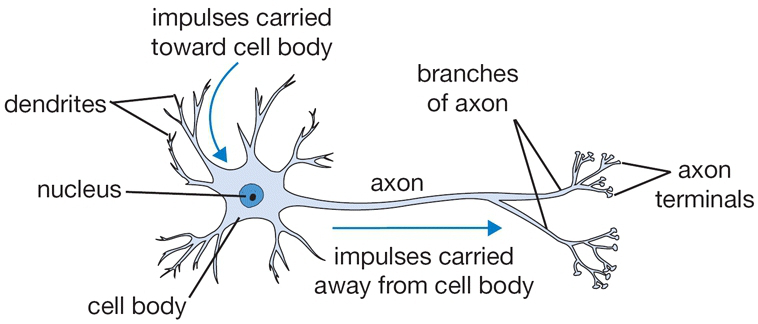
\includegraphics[width=8cm]{figuras/neuron}
\caption{Representação de um neurônio biológico.\footnote{Extraído de \url{https://cs231n.github.io/neural-networks-1/}}}
\label{fig:neuron}
\end{figure}

Dá-se o nome de \eng{perceptron} de camada única (\eng{single-layer perceptron}) ou simplesmente \eng{perceptron} a uma das simples arquiteturas de rede neural artificial, criada em 1957 por Frank Rosenblatt \citep{frank}. Uma ilustração conceitual dela está na figura~\ref{fig:perceptron}. Existem atualmente diversas outras arquiteturas de redes neurais, mas a extensão mais imediata que podemos citar de um perceptron constituído de uma camada de neurônios são as redes \eng{perceptron} multi-camadas (\eng{multi-layer perceptron}). 

Os neurônios são representados por círculos, dentro deles há um valor numérico que intuitivamente podemos atribuir ao nível ou grau de ativação do neurônio, mesmo que no caso biológico se restrinja aos valores $0$ e $1$, ou seja, ativados ou não. Cada coluna de neurônios representa uma camada, nesse caso, da esquerda para a direita temos a camada de entrada, a camada oculta e a camada de saída. As linhas representam as ligações entre os neurônios, sendo que cada neurônio de uma camada está ligado a todos da camada anterior.

\begin{figure}[htb]
\centering
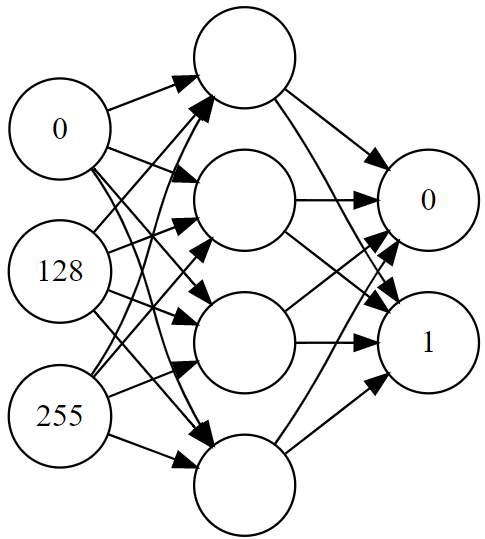
\includegraphics[width=5cm]{figuras/perceptron}
\caption{Rede neural simples, o perceptron de camada única.}
\label{fig:perceptron}
\end{figure}

O perceptron de camada única consiste de uma camada de neurônios de entrada, uma camada oculta de neurônios usados na otimização, e uma camada de saída, que irá conter os dados previstos, ou ainda as probabilidades do dado pertencer a alguma das classes que a rede poderá classificá-lo. E é o fato de haver uma camada oculta nesta rede que a define como sendo de ``camada única''. Caso houvessem mais do que uma camada oculta, ela seria do tipo ``multi-camadas'' mencionada acima.

De modo a entendermos as bases matemáticas do algoritmo, podemos começar de uma rede ainda mais básica, a partir um \eng{perceptron} que seja constituído de apenas $1$ neurônio na única camada oculta. Esta rede super simplificada, que está na figura~\ref{fig:neuronio}, pode ser útil para para o entendimento uma vez que neste caso será possível acompanhar graficamente o resultado da execução do algoritmo.

\begin{figure}[htb]
\centering
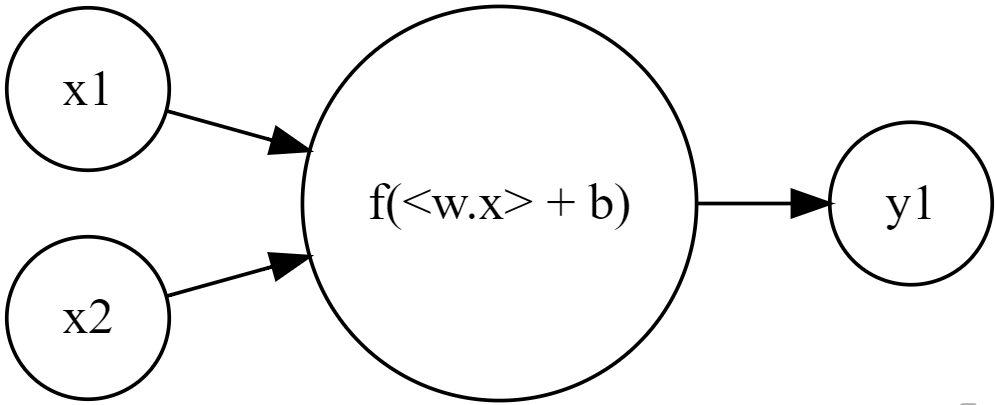
\includegraphics[width=8cm]{figuras/neuronio}
\caption{Rede neural mais simples ainda, apenas um neurônio oculto.}
\label{fig:neuronio}
\end{figure}

Esta rede possui $2$ neurônios na camada de entrada, que são os números reais $x_1$ e $x_2$, $1$ neurônio na camada oculta, no qual está a sua função de ativação $f(x_1w_1 + x_2w_2 + b)$, e $1$ neurônio na camada de saída, que neste caso é um número real $y_1$. Pode-se notar a semelhança dessa rede neural artificial com a sua inspiração biológica com a ajuda da figura~\ref{fig:neuron_model}. 

\begin{figure}[htb]
\centering
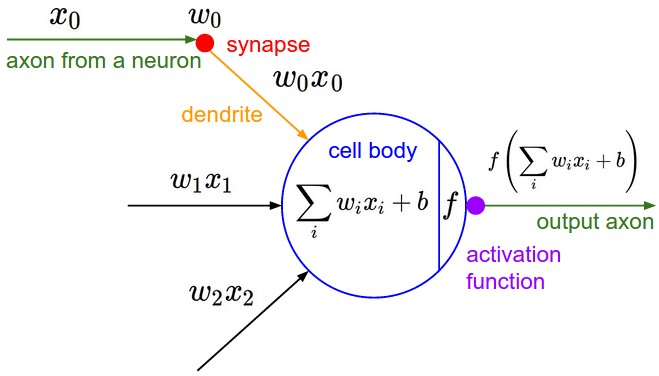
\includegraphics[width=8cm]{figuras/neuron_model}
\caption{Representação de um neurônio artificial.\footnote{Extraído de \url{https://cs231n.github.io/neural-networks-1/}}}
\label{fig:neuron_model}
\end{figure}

Temos os sinais de entrada (como o $x_1$) vindos como viriam os sinais dos axônios de outros neurônios. Eles entram pela camada de entrada da rede, ou dentritos do neurônio. A camada oculta processa as entradas com os pesos, definindo o formato final do sinal através de sua função de ativação, que aqui pode ser uma função real qualquer, mas com funcionalidade similar ao do núcleo do neurônio que ativa/transmite ou não o sinal recebido por ele. Por fim o sinal é enviado à camada de saída, ou aos axônios do neurônio, concluíndo o processamento.

A partir desta analogia podemos compreender o funcionamento básico da rede artificial \eng{perceptron}. Ela recebe uma lista de valores como entrada, que podemos representar por um vetor real $x$. O neurônio oculto representa uma transformação linear neste vetor, que podemos escrever como o produto escalar por um outro vetor real, o vetor de \defi{pesos} $w$, ou seja, $<w.x>$, que é o produto escalar usual dos números reais. A seguir, somamos um outro número real $b$ que é chamado de \defi{viés}, que possui o mesmo papel que a constante de interceptação da reta com o eixo vertical de um ajuste linear.

Por fim, é aplicada uma função de ativação não-linear sobre esta transformação, o que configura a saída deste neurônio: $f({<w.x>} + b)$, que é transmitida ao neurônio de saída, que pode aplicar uma transformação semelhante ou outra qualquer, dependendo da função de ativação utilizada em cada camada da rede. Por simplicidade mostramos uma rede bem simples, mas na prática podem haver muito mais camadas ocultas, e cada uma delas assim como a camada de saída, podem ter muitos neurônios cada.

Este processo de entrada, processamento e saída da rede é chamado de \defi{feedforward}, e consiste no nível mais fundamental do \eng{perceptron}. A partir daí, a forma como a rede será treinada, é o que define se ela será utilizada para um aprendizado supervisionado ou não-supervisionado.

Uma vez que estamos lidando com o aprendizado supervisionado, dever ser utilizado um algoritmo de treinamento que forneça à rede pares conhecidos de vetores de entradas e saídas esperadas, e um \defi{critério de avaliação} de quão boa é a performance da rede para aproximar as suas saídas das saídas esperadas. 

Este critério é uma função que fornece uma medida da distância entre as saídas obtidas pela rede e as saídas esperadas, que é genericamente chamada de função de custo (\eng{cost function}). Se denotarmos por $y$ uma saída conhecida, e por $a^{(L)}$ uma saída obtida pela última camada, exemplos comumente usados são as normas usuais como a distância euclidiana ($(a^{(L)^2} + y^2)^{1/2}$), a função de erro absoluto ($|a^{(L)} - y|$), e a função de erro quadrático médio ($(a^{(L)} - y)^2$) , (\eng{mean square error}, MSE), que é a usada no algoritmo descrito por Kopec \citep{classic} e que será usado neste trabalho.

Um dos algoritmos de treinamento que minimizam uma função de custo é o gradiente descendente (\eng{gradient descent}), que segundo Géron \citep{hands} é um algoritmo muito geral e que serve para encontrar soluções ótimas para uma grande variedade de problemas de otimização. Detalhes de seu funcionamento podem ser vistos no Apêndice \ref{ap:gradiente}.

\section{Outras arquiteturas de redes neurais}

Existem dezenas de arquiteturas de redes neurais artificiais, uma breve olhada na quantidade de arquiteturas listadas no website \emph{The neural network zoo}\footnote{\url{https://www.asimovinstitute.org/neural-network-zoo/}} demonstra que essa brincadeira é levada muito a sério. A representação gráfica ali criada é útil para o entendimento das características das diversas arquiteturas, graças aos padrões de cores e de formas geométricas utilizadas.

A primeira estrutura é o \eng{perceptron} simples, de apenas um neurônio, que processa $n$ entradas através de uma transformação linear seguida de uma função de ativação. É exibido no canto superior esquerdo da Figura \ref{fig:estrutura_p}.

\begin{figure}[htb]
\centering
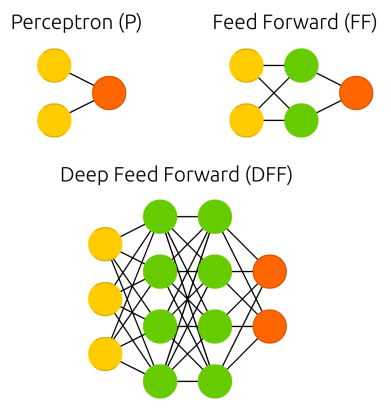
\includegraphics[width=7cm]{figuras/estrutura_p}
\caption{As redes neurais recorrentes: \eng{perceptron}, \eng{feedforward} e \eng{deep feedforward}.\footnote{Extraído de \url{https://www.asimovinstitute.org/neural-network-zoo/}}}
\label{fig:estrutura_p}
\end{figure}

No canto superior direito está a versão \eng{feedforward}, possuindo uma camada oculta(representada pelos círculos verdes), e embaixo está a versão \eng{deep feedforward}, que possui múltiplas camadas ocultas, e número variado de neurônios em todas as camadas, e é de fato a versão que foi implementada nesse trabalho.

As características em comum das arquiteturas derivadas da rede \eng{perceptron}, chamadas de \defi{redes neurais sequenciais}, são a conexão que existe entre cada neurônios de uma camada com todos os neurônios da camada anterior, e a forma que a informação é transmitida da rede, num sentido único, da camada de entrada(os círculos amarelos) para a camada de saída(os círculos vermelhos).

A próxima arquitetura em destaque define o que são as \defi{redes neurais recorrentes}, ilustrada na Figura \ref{fig:estrutura_r}. Nesse tipo de rede a informação pode ir para frente e para trás, além disso pode passar pelo mesmo neurônio oculto mais de uma vez, o que determina o nome recorrente. Esses neurônios são representados pela cor azul na figura.

\begin{figure}[htb]
\centering
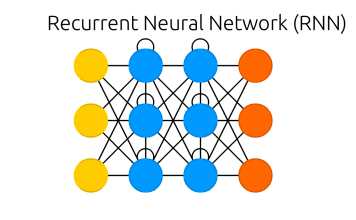
\includegraphics[width=7cm]{figuras/estrutura_r}
\caption{As redes neurais recorrentes.\footnote{Extraído de \url{https://www.asimovinstitute.org/neural-network-zoo/}}}
\label{fig:estrutura_r}
\end{figure}

Esse tipo de rede, segundo Kopec \citep{classic} é o mais usado em problemas em que os dados utilizados possuem uma dependência da ordem em que são obtidos e possuem entradas contínuas, por exemplo, os dados de uma série temporal de dados, ou seja, em que a previsão de um dado , o que representaria o futuro, depende da ordem em que estão os dados já conhecidos, o que representaria os dados do passado.

Outra arquitetura muito utilizada é o das \defi{redes neurais covolucionais}, ilustradas na Figura \ref{fig:estrutura_c}.  Segundo Kopec \citep{classic} essas redes foram projetadas e usadas com sucesso para classificação de imagens ``pesadas'', como fotos de galáxias obtidas em telescópios.

\begin{figure}[htb]
\centering
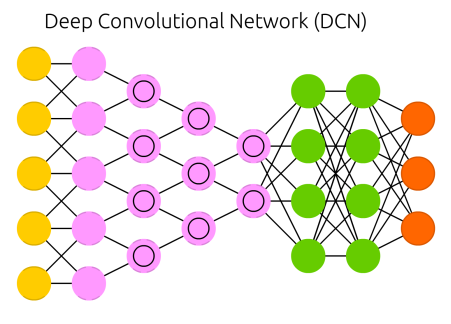
\includegraphics[width=8cm]{figuras/estrutura_c}
\caption{As redes neurais convolucionais.\footnote{Extraído de \url{https://www.asimovinstitute.org/neural-network-zoo/}}}
\label{fig:estrutura_c}
\end{figure}

Em resumo, são redes em que os neurônios de entrada não são conectados totalmente com a primeira camada oculta, mas o que acontece é que vários conjuntos distintos de neurônios da camada de entrada são conectados a várias camadas ocultas separadamente.

A seguir a união dessas camadas ocultas, exibidas como círculos rosas, conectam-se em cascata, perdendo conexões progressivamente até que um número reduzido se conecta a outras camadas, dessa vez camadas ocultas simples, que são os círculos verdes, que conectam-se em formato \eng{feedforward} até o final da rede com a camada de saída. 

Existem ainda outras dezenas de arquiteturas, algumas bem alternativas no formato e nas conexões entre as camadas, fica aqui um único exemplo dentre elas, que é a arquitetura de \defi{redes neurais extremas}. Está ilustrada na Figura \ref{fig:estrutura_e}.

\begin{figure}[htb]
\centering
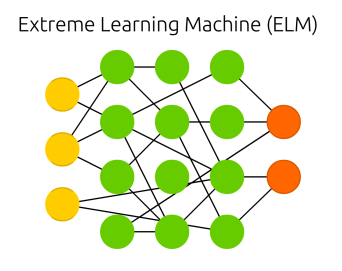
\includegraphics[width=7cm]{figuras/estrutura_e}
\caption{Redes neurais extremas.\footnote{Extraído de \url{https://www.asimovinstitute.org/neural-network-zoo/}}}
\label{fig:estrutura_e}
\end{figure}

As conexões ocorrem de forma não-sequencial, e até mesmo aleatória entre as camadas ocultas, configurando um exemplo curioso de arquitetura, e discussões sobre essas outras arquiteturas não fazem parte do escopo desse trabalho.